\documentclass{article}
\usepackage{graphicx}
\title{Q Vector Computation}
\author{Carlos Perez Lara\and Jaehyeon Do \and Veronica Canoa Roman}
\date{Last updated: \today}

\begin{document}
\maketitle

\section{Definitions}
%===================Q Vector
The {\bf Q vector} is an event-by-event observable defined as
\begin{equation}
\label{eq.q}
Q_n = \sum_{i} \omega_i e^{i n\varphi_i} = \vert Q_n \vert e^{i n\Psi_n}
\end{equation}
where he sum goes over all particles in the sample and $\varphi_i$ is the laboratory azimuthal angle of the particles emerging from the collision.
When the sample is composed of reconstructed particles, the weight $\omega_i$  is sometimes different than 1 in order to enhance the contribution of particles with the highest contribution to the flow, on the other hand, for some detector configurations (like BBC, FVTX and MPCEX) the weight $\omega_i$ is the relative energy flow.

The {\bf symmetry angle} $\Psi_n$ is the angle associated to the Q vector and is defined in equation \ref{eq.q}.

\section{Correcting Q$_n$ against biases}
The Q vector can be computed by any detector that has azimuthal granularity (trackers, hodoscopes, calorimeters, etc).
For a proper unbiased estimator, one need to correct by detector non-uniform acceptance and efficiency.
The corrections used here are computed from the data itself and consist of several steps (more information on these methods can be found in \cite{PhysRevC.77.034904,PhysRevC.56.3254}):

{\bf 1. Recentering the Q centroid.}
\begin{equation}
Q^\mathrm{I}_{nx} = Q_{nx}(1-\langle \cos{n\varphi}\rangle), \qquad
Q^\mathrm{I}_{ny} = Q_{ny}(1-\langle \sin{n\varphi}\rangle)
\end{equation}

{\bf 2. Twist of the Q vector.}
\begin{equation}
Q^\mathrm{II}_{nx} = \frac{Q^\mathrm{I}_{nx}-\lambda^{s-}_{2n} Q^\mathrm{I}_{ny}}{1-\lambda^{s-}_{2n}\lambda^{s+}_{2n}}, \,
Q^\mathrm{II}_{ny} = \frac{Q^\mathrm{I}_{ny}-\lambda^{s+}_{2n} Q^\mathrm{I}_{nx}}{1-\lambda^{s-}_{2n}\lambda^{s+}_{2n}}, \,
\lambda^{s\pm}_{2n}=\frac{\langle\sin{2n\varphi}\rangle}{1\pm\langle\cos{2n\varphi}\rangle}
\end{equation}

{\bf 3. Scaling the Q vector.}
\begin{equation}
Q^\mathrm{III}_{nx} = \frac{Q^\mathrm{II}_{nx}}{1+\langle\cos{2n\varphi}\rangle}, \qquad
Q^\mathrm{III}_{ny} = \frac{Q^\mathrm{II}_{ny}}{1-\langle\cos{2n\varphi}\rangle}
\end{equation}

{\bf 4. Flattening the symmetry angle.}
\begin{equation}
\Psi^\mathrm{IV}_{n} = \Psi^\mathrm{III}_{n} + \sum_{m}\frac{2}{m}( -\langle\sin{m\Psi^\mathrm{III}_n}\rangle\cos{m\Psi^\mathrm{III}_n} +\langle\cos{m\Psi^\mathrm{III}_n}\rangle\sin{m\Psi^\mathrm{III}_n})
\end{equation}

Each of these effects were corrected sequentially, which requires several passes over data. Notice that if there were not any bias, each of the averages "$\langle\rangle$" would be zero and thus $Q^\mathrm{IV}=Q^\mathrm{III}=Q^\mathrm{II}=Q^\mathrm{I}=Q$ we recover the original Q.

\section{BBC Q$_n$ vectors}
\begin{figure}
\label{fig.bbcgeo}
\caption{Geometrical sketch of the BBC south arm sub-detectors}
\end{figure}
The BBC detector consist of two arrays of detectors, each covering either $-2.9<\eta<-2.1$ (north) or $2.1<\eta<2.9$ (south).
Each arm consists of 64 detectors. Figure \ref{fig.bbcgeo} depicts the geometrical arrange in the x-y plane for the south arm.
Following equation \ref{eq.q} the BBC-based Q vectors can be constructed expanding the sum over the 64 detectors and using the center of each detector for the determination of $\varphi_i$ and the calibrated ADC signal of each detector as weight $\omega_i$.

{\bf Q$_n$ accuracy.}
The BBC accuracy for the measured Q vector can be quantified by measuring the resolution of its $\Psi_n$ counterpart.
There are several methods to do that. In this analysis we rely on measuring the resolution of the detector by using subevents within the same detector. This is done in order to prevent using other detector with different detector azimuthal non-uniformities or, worse yet, the coupling of longitudinal expansion effects.
For the BBC this can be done since each arm side can be separated into two independent sub-detector each equally sensitive to the event multiplicity and its flow and having approximately the same geometrical configuration.
The resolution can then be computed using the methods in \cite{PhysRevC.77.034904}. Namely for the strongest contribution:
\begin{equation}
\langle\cos{n(\Psi_n-\Psi)}\rangle = \frac{\sqrt{\pi}}{2\sqrt{2}}\chi_n e^{-\chi_n^2/4}\lbrace I_0(\chi_n^2/4)-I_1(\chi_n^2/4)\rbrace
\end{equation}

\section{Run16 dAu 200 GeV}
\begin{figure}
\centering
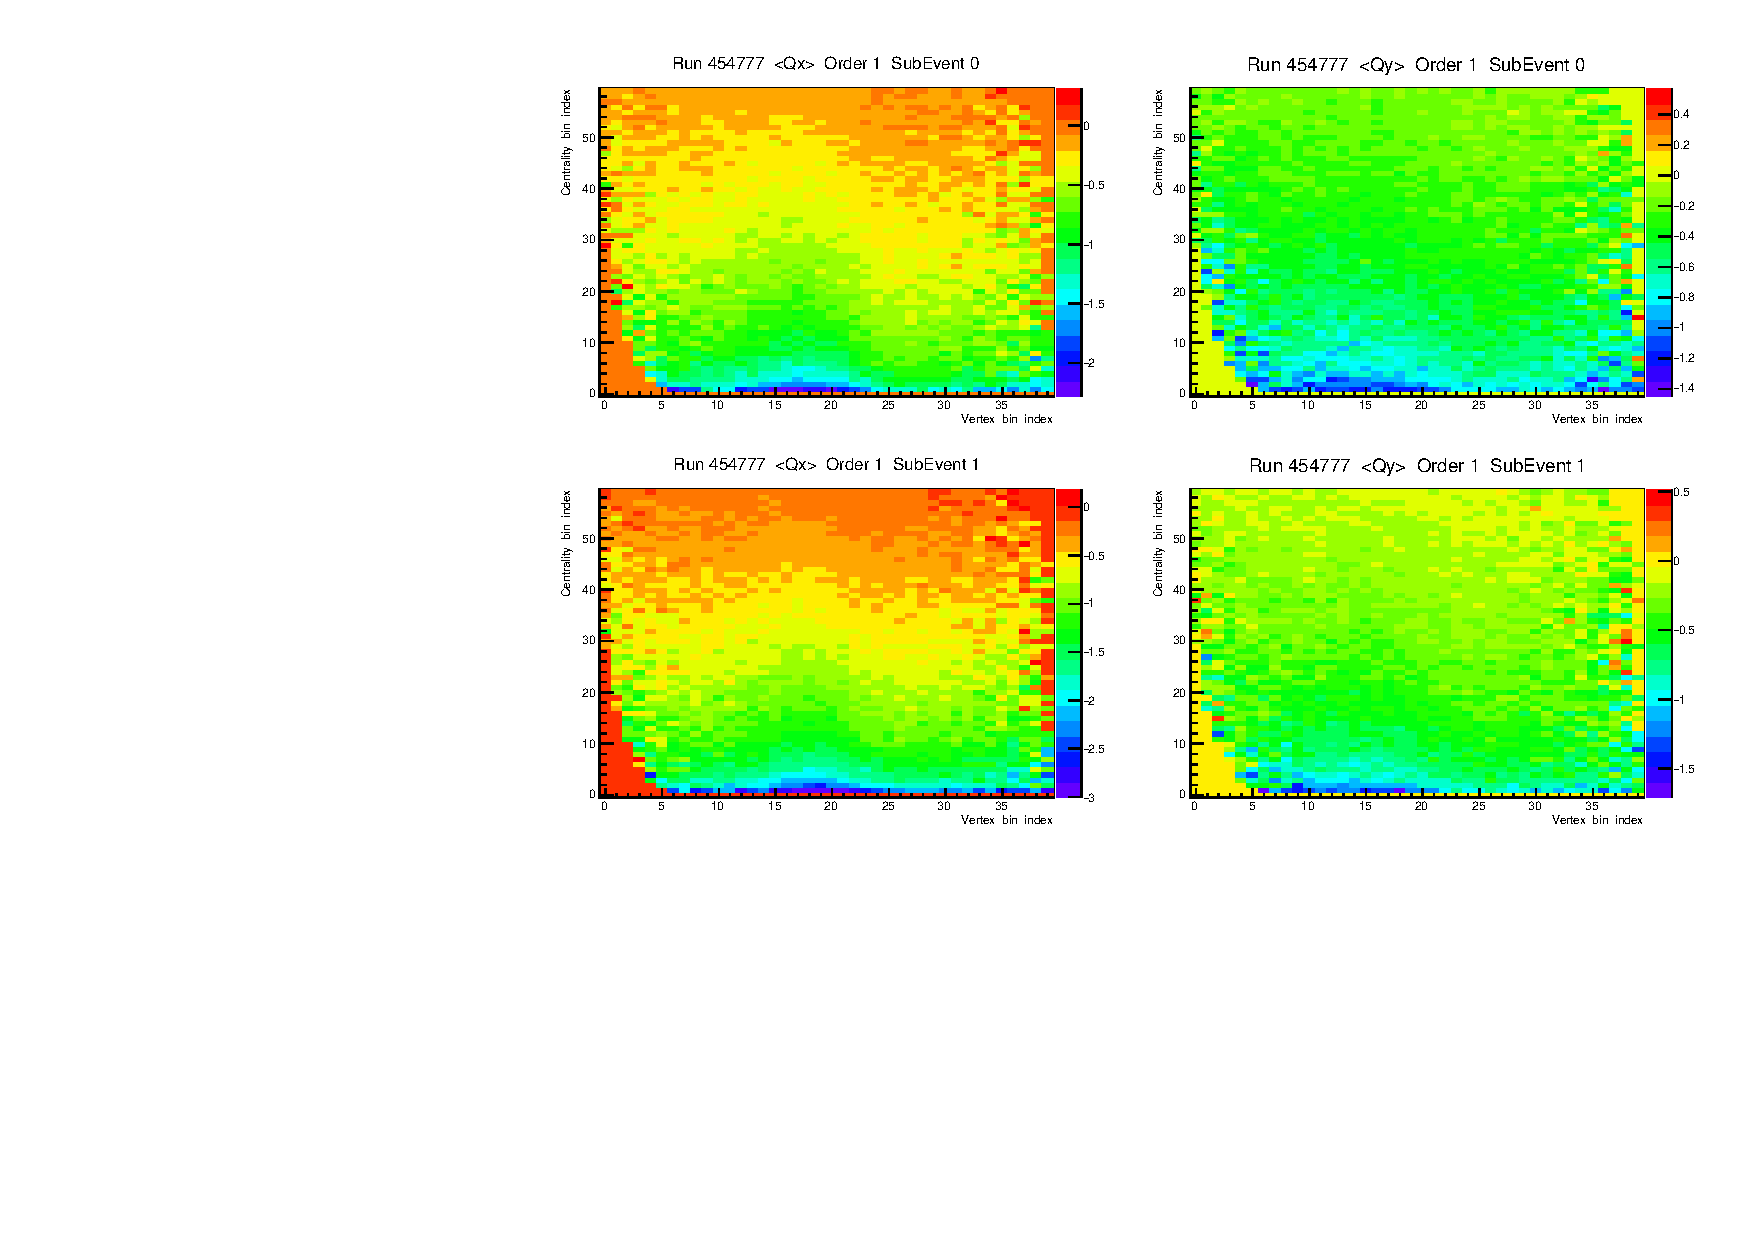
\includegraphics[width=0.7\textwidth]{fig_eventplane/QC_454777_ORD0.pdf}
\label{fig.bbc.qc0}
\caption{Non-normalized coefficients for Q$_1$ vector centering for BBC Run 454777 as a function of centrality and vertex bin. The top panels correspond to subevent 0 and the bottom panels correspond to subevent 1. The nominal vertex z=0 sits at around bin index 20 in the X axis.}
\end{figure}
\begin{figure}
\centering
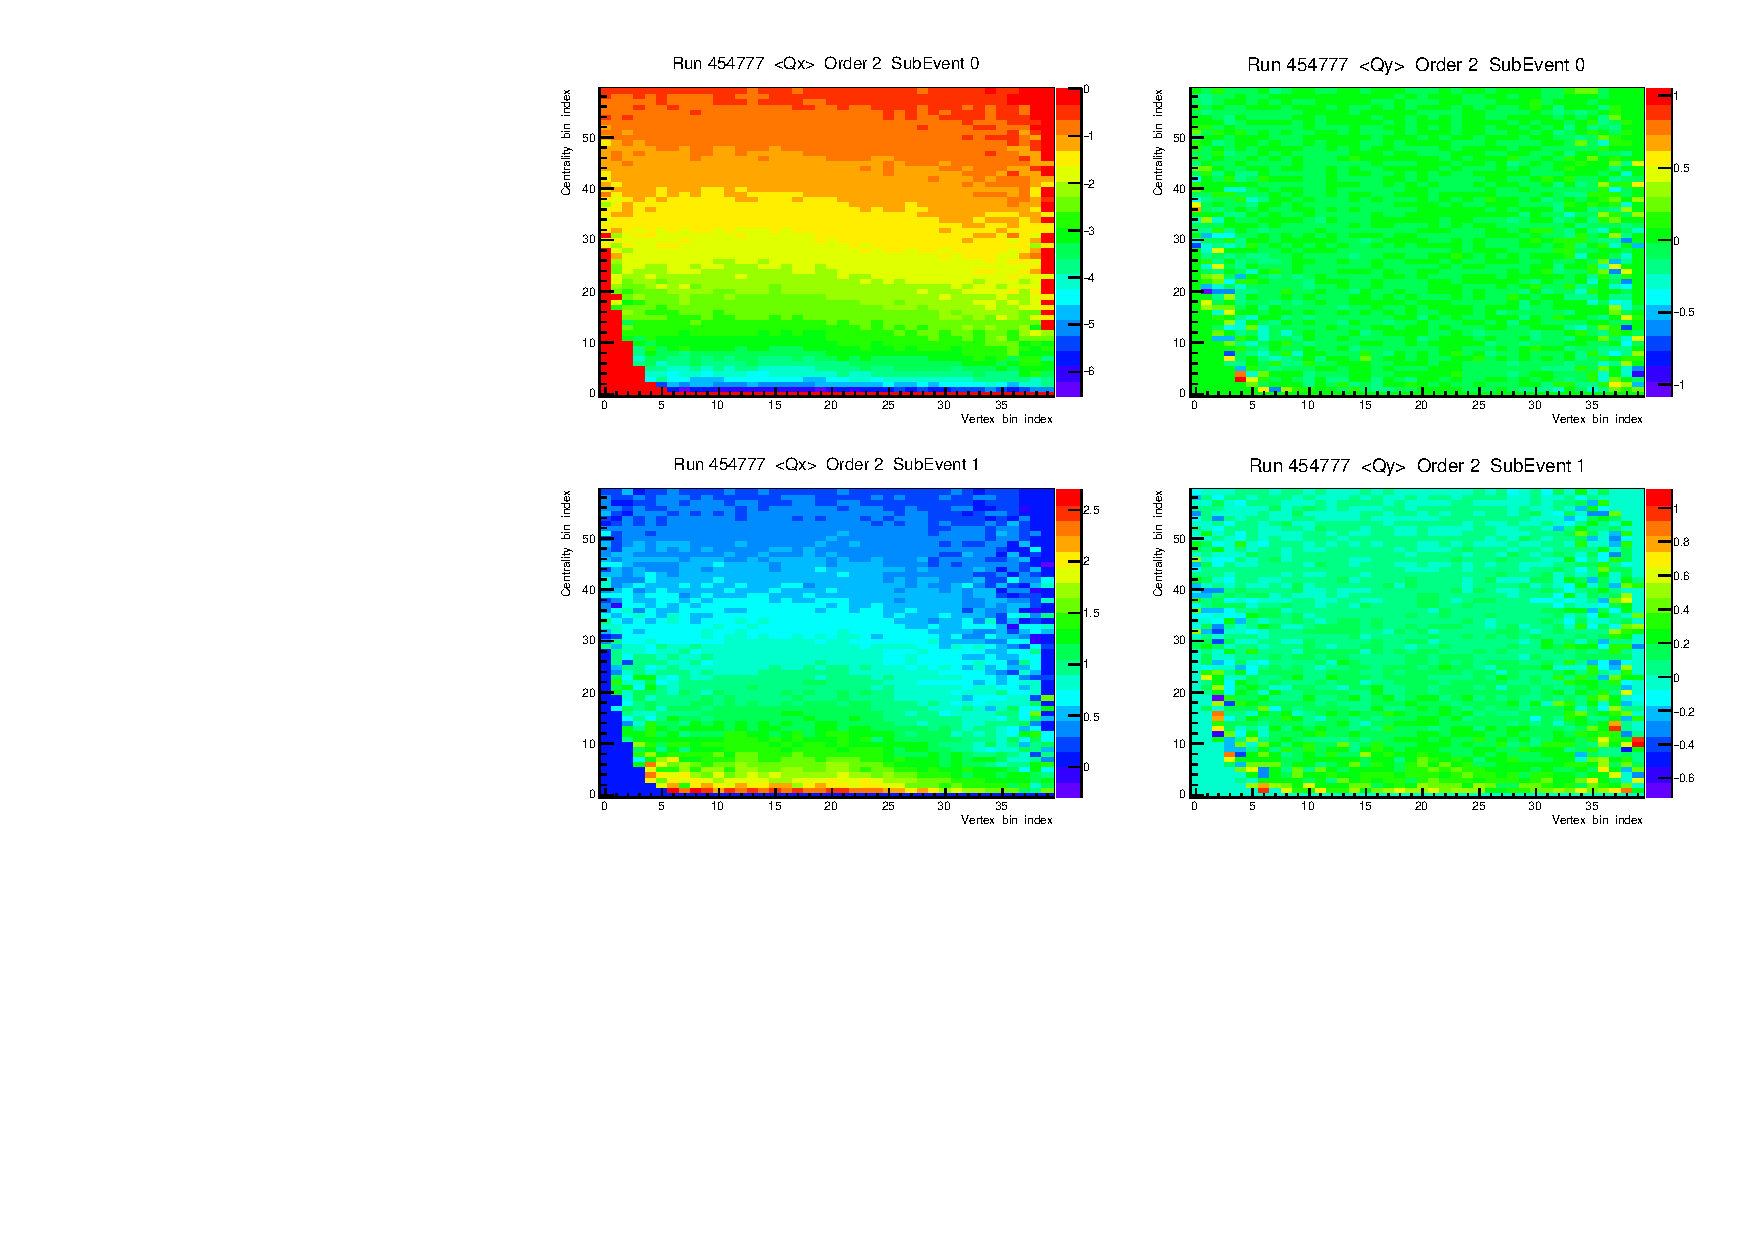
\includegraphics[width=0.7\textwidth]{fig_eventplane/QC_454777_ORD1.pdf}
\label{fig.bbc.qc1}
\caption{Non-normalized coefficients for Q$_2$ vector centering for BBC Run 454777 as a function of centrality and vertex bin. The top panels correspond to subevent 0 and the bottom panels correspond to subevent 1. The nominal vertex z=0 sits at around bin index 20 in the X axis.}
\end{figure}
\begin{figure}
\centering
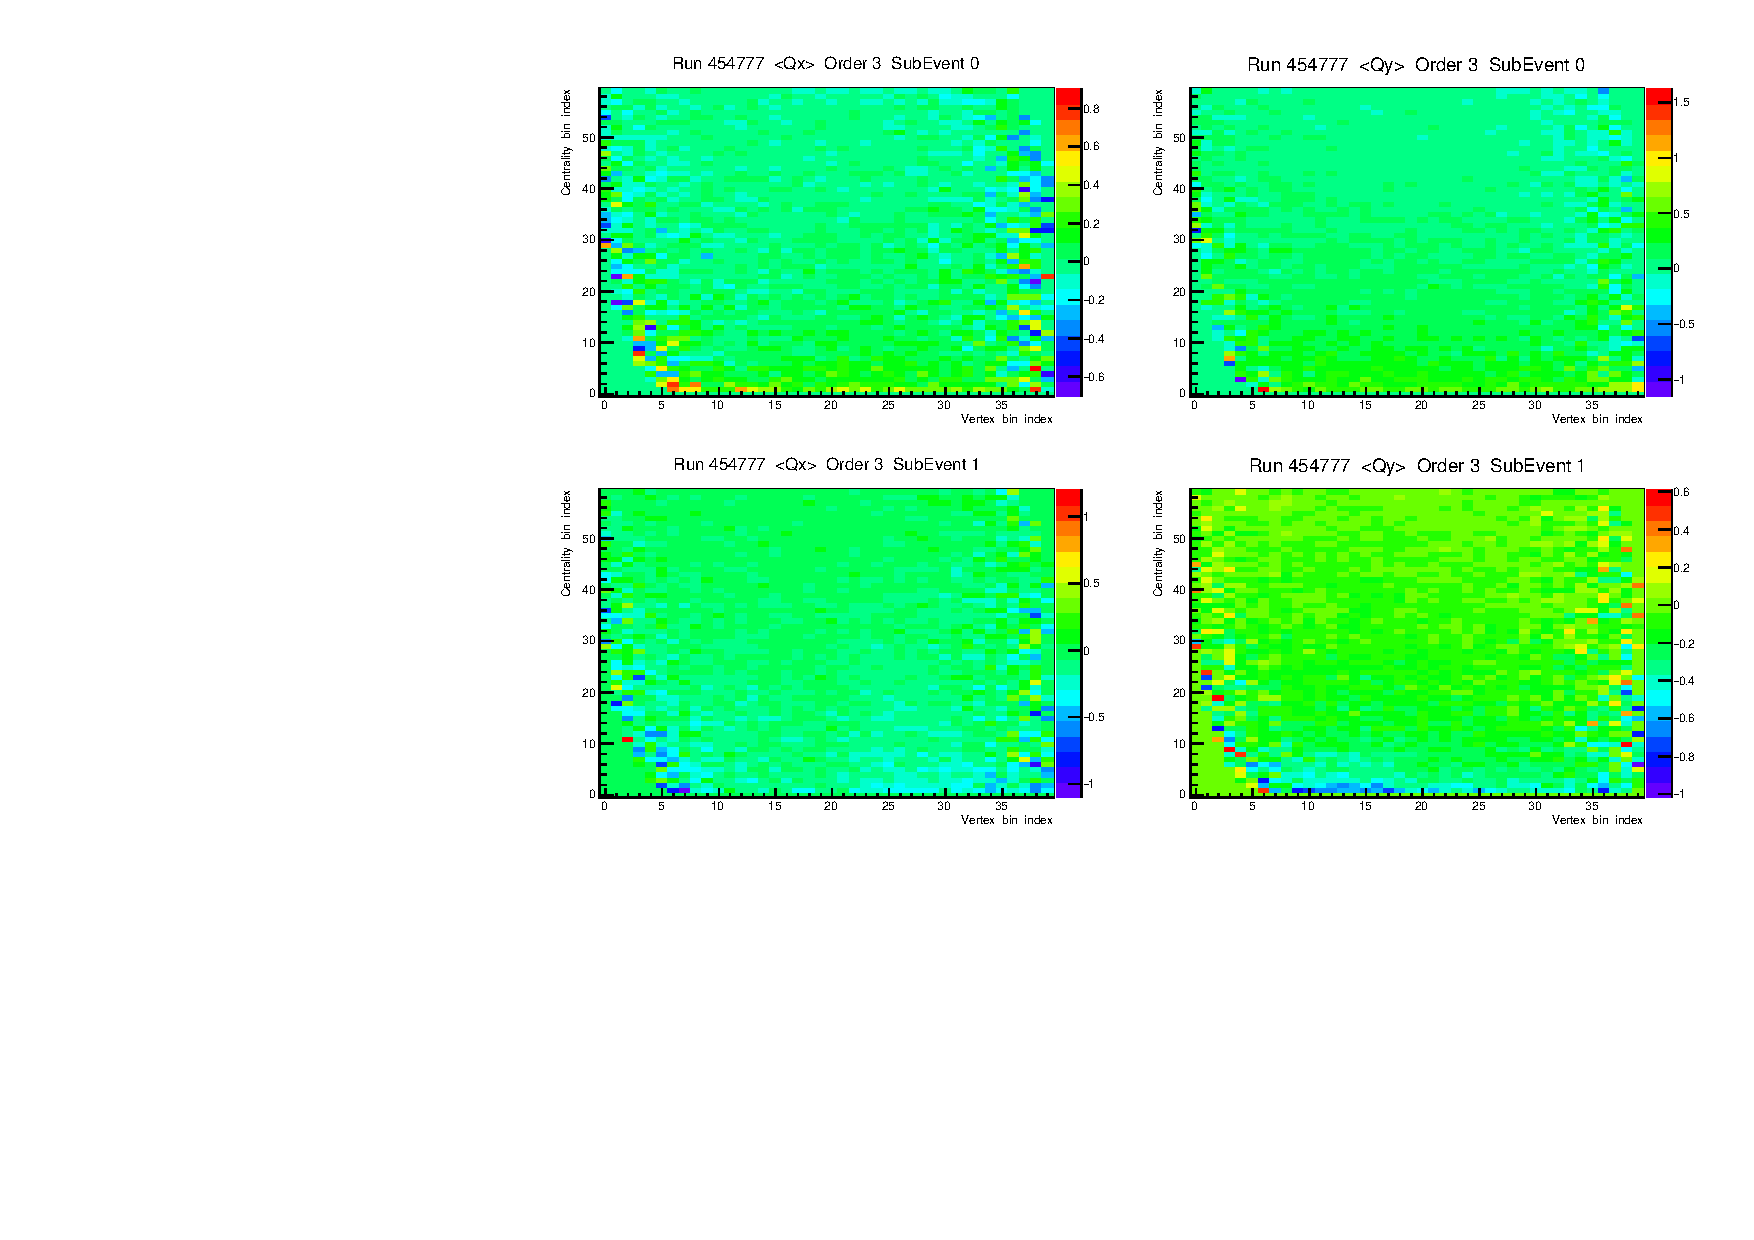
\includegraphics[width=0.7\textwidth]{fig_eventplane/QC_454777_ORD2.pdf}
\label{fig.bbc.qc2}
\caption{Non-normalized coefficients for Q$_3$ vector centering for BBC Run 454777 as a function of centrality and vertex bin. The top panels correspond to subevent 0 and the bottom panels correspond to subevent 1. The nominal vertex z=0 sits at around bin index 20 in the X axis.}
\end{figure}
\begin{figure}
\centering
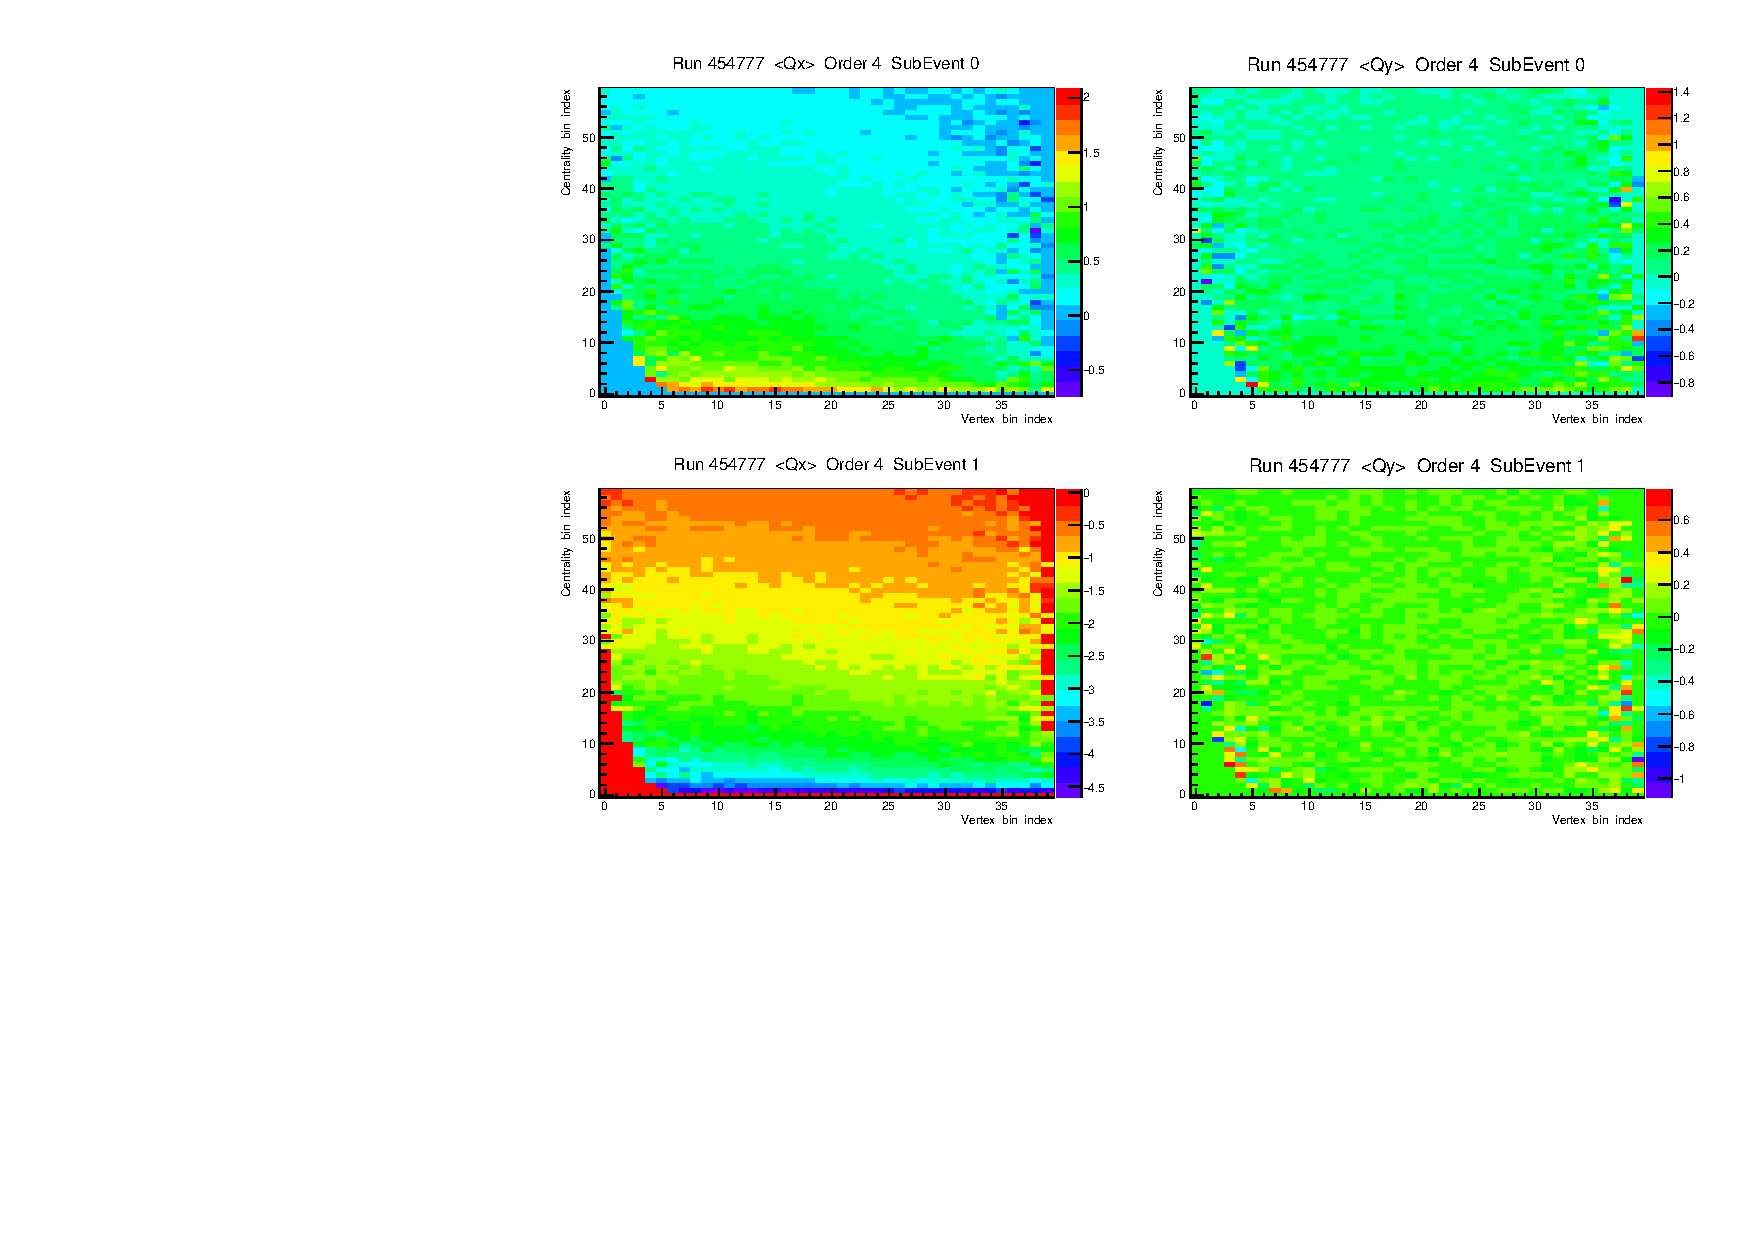
\includegraphics[width=0.7\textwidth]{fig_eventplane/QC_454777_ORD3.pdf}
\label{fig.bbc.qc3}
\caption{Non-normalized coefficients for Q$_4$ vector centering for BBC Run 454777 as a function of centrality and vertex bin. The top panels correspond to subevent 0 and the bottom panels correspond to subevent 1. The nominal vertex z=0 sits at around bin index 20 in the X axis.}
\end{figure}
\begin{figure}
\centering
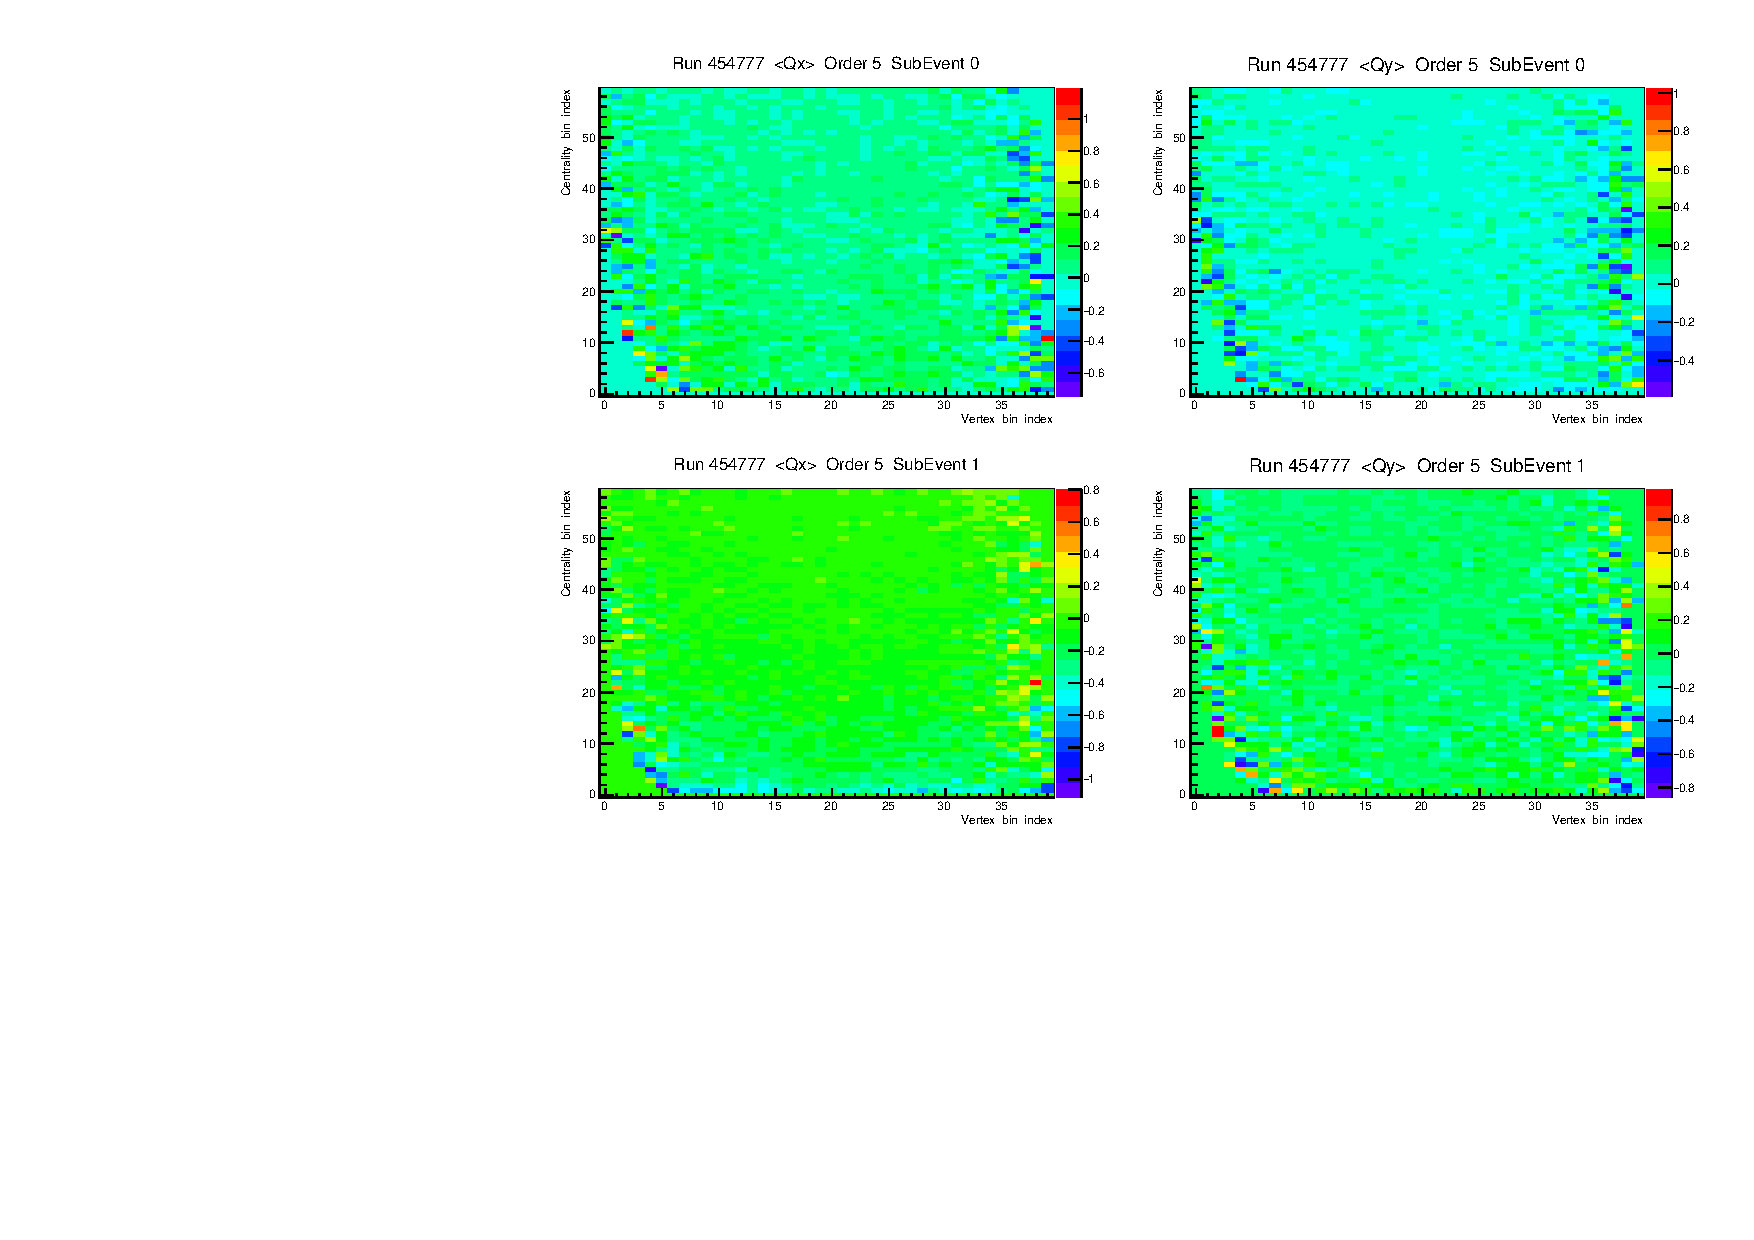
\includegraphics[width=0.7\textwidth]{fig_eventplane/QC_454777_ORD4.pdf}
\label{fig.bbc.qc4}
\caption{Non-normalized coefficients for Q$_5$ vector centering for BBC Run 454777 as a function of centrality and vertex bin. The top panels correspond to subevent 0 and the bottom panels correspond to subevent 1. The nominal vertex z=0 sits at around bin index 20 in the X axis.}
\end{figure}
\begin{figure}
\centering
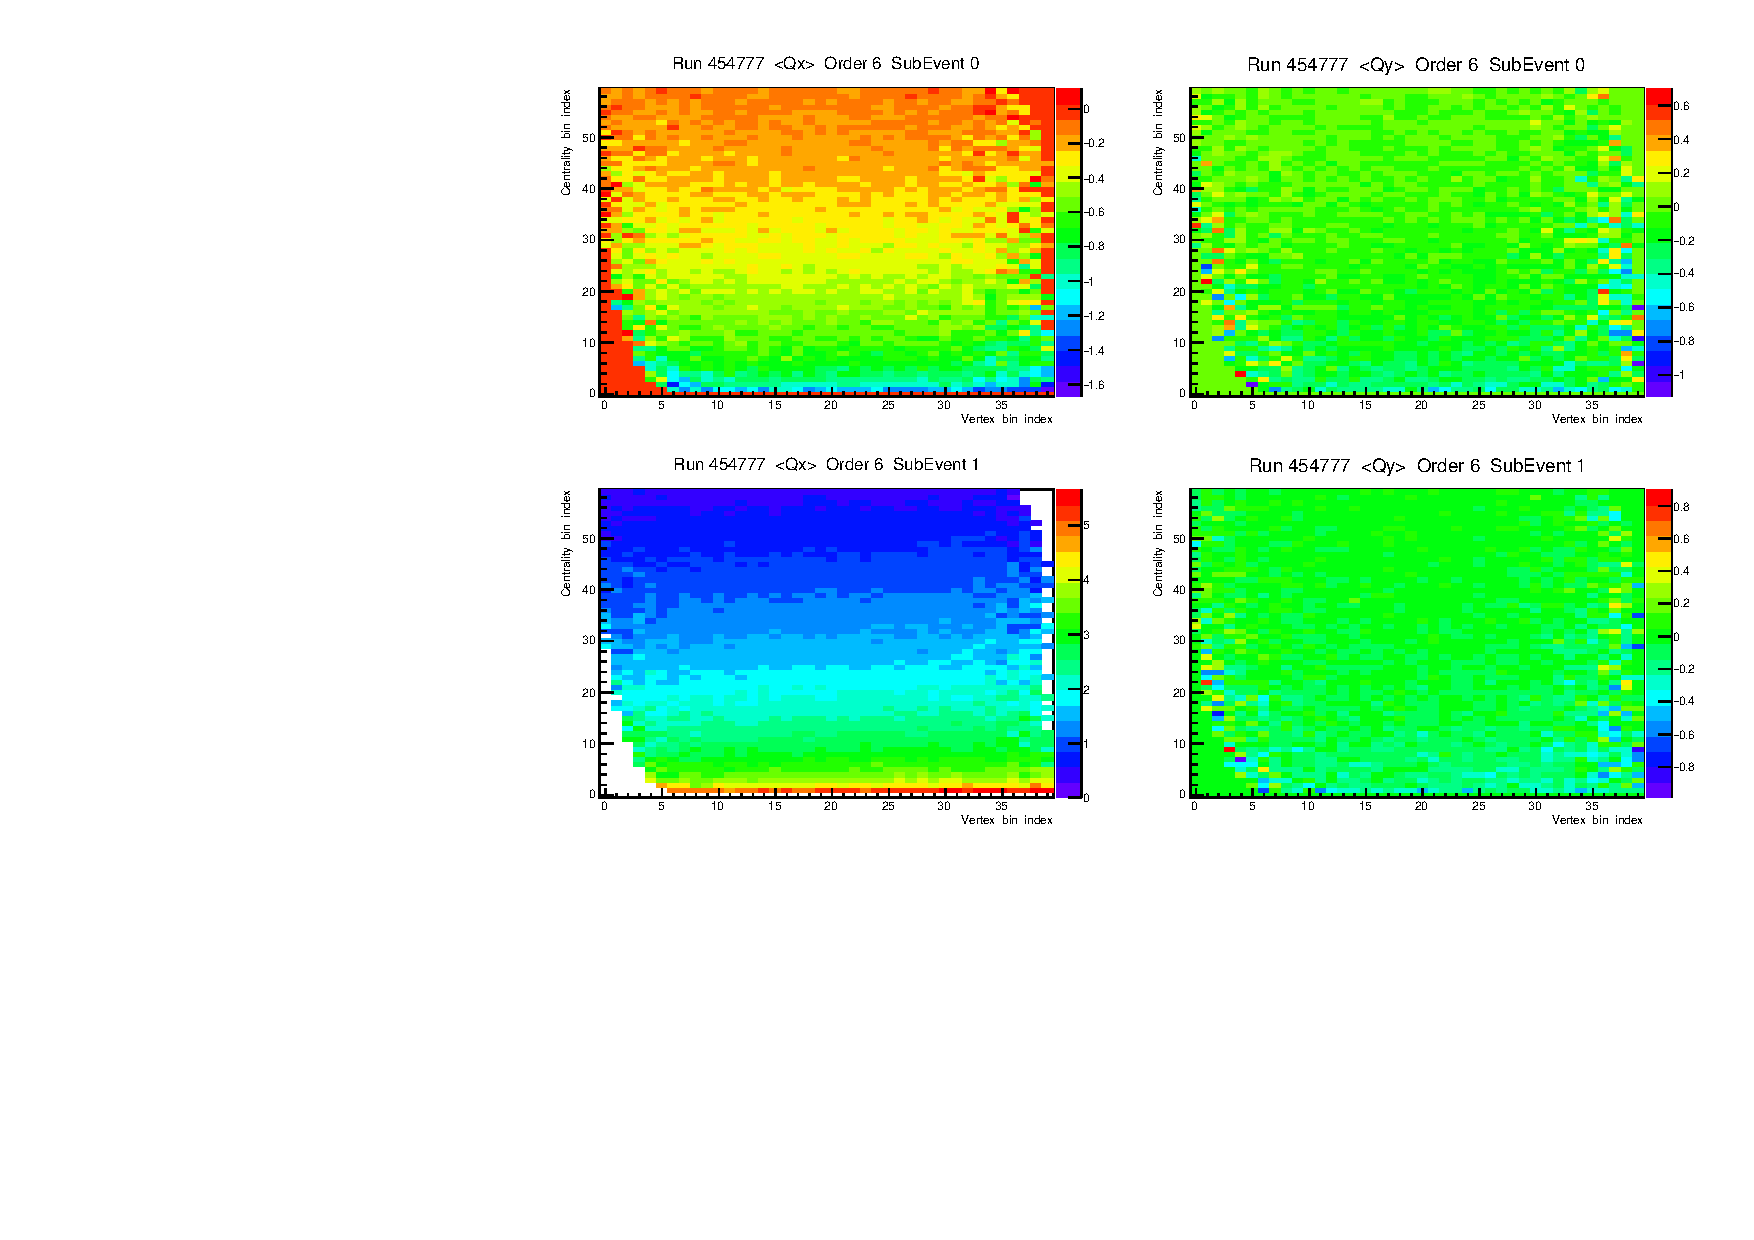
\includegraphics[width=0.7\textwidth]{fig_eventplane/QC_454777_ORD5.pdf}
\label{fig.bbc.qc5}
\caption{Non-normalized coefficients for Q$_6$ vector centering for BBC Run 454777 as a function of centrality and vertex bin. The top panels correspond to subevent 0 and the bottom panels correspond to subevent 1. The nominal vertex z=0 sits at around bin index 20 in the X axis.}
\end{figure}
\begin{figure}
\centering
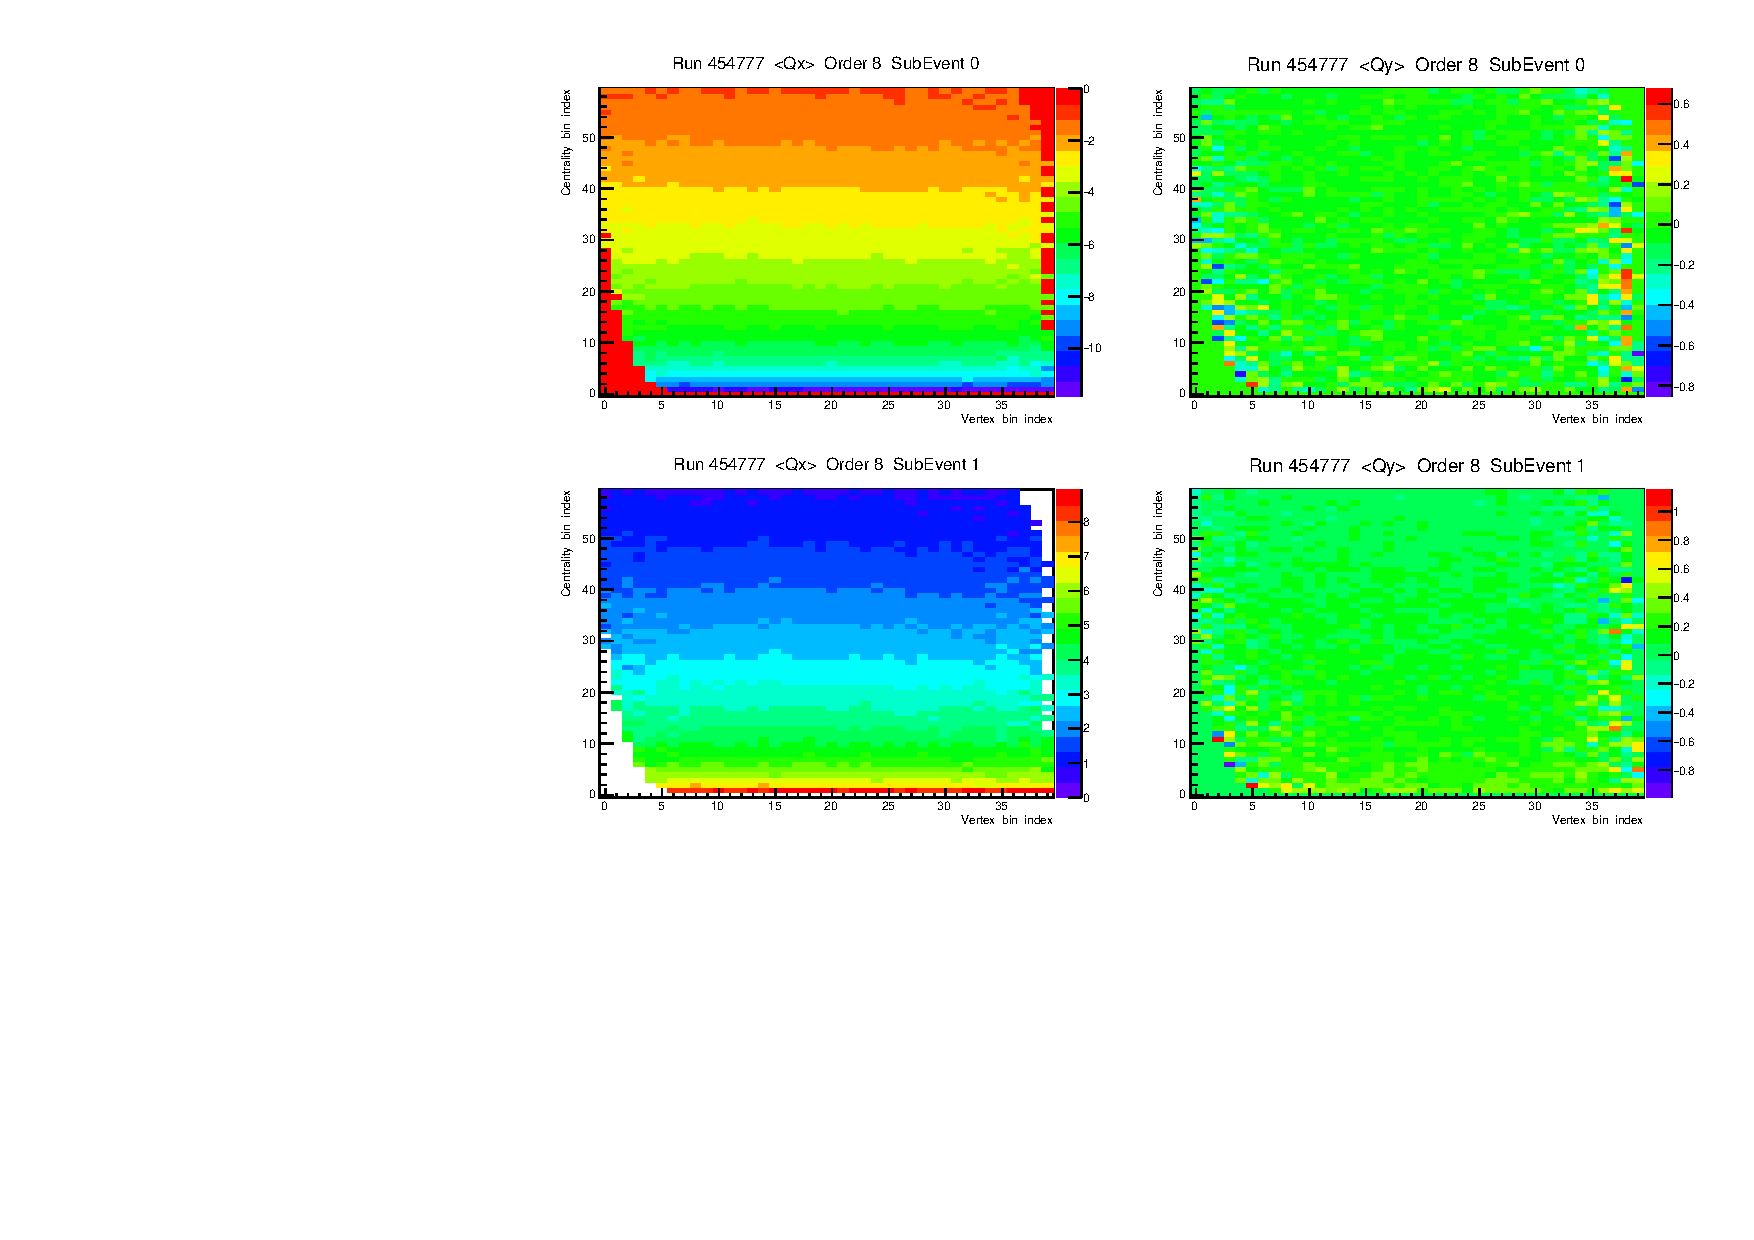
\includegraphics[width=0.7\textwidth]{fig_eventplane/QC_454777_ORD6.pdf}
\label{fig.bbc.qc6}
\caption{Non-normalized coefficients for Q$_8$ vector centering for BBC Run 454777 as a function of centrality and vertex bin. The top panels correspond to subevent 0 and the bottom panels correspond to subevent 1. The nominal vertex z=0 sits at around bin index 20 in the X axis.}
\end{figure}
\begin{figure}
\centering
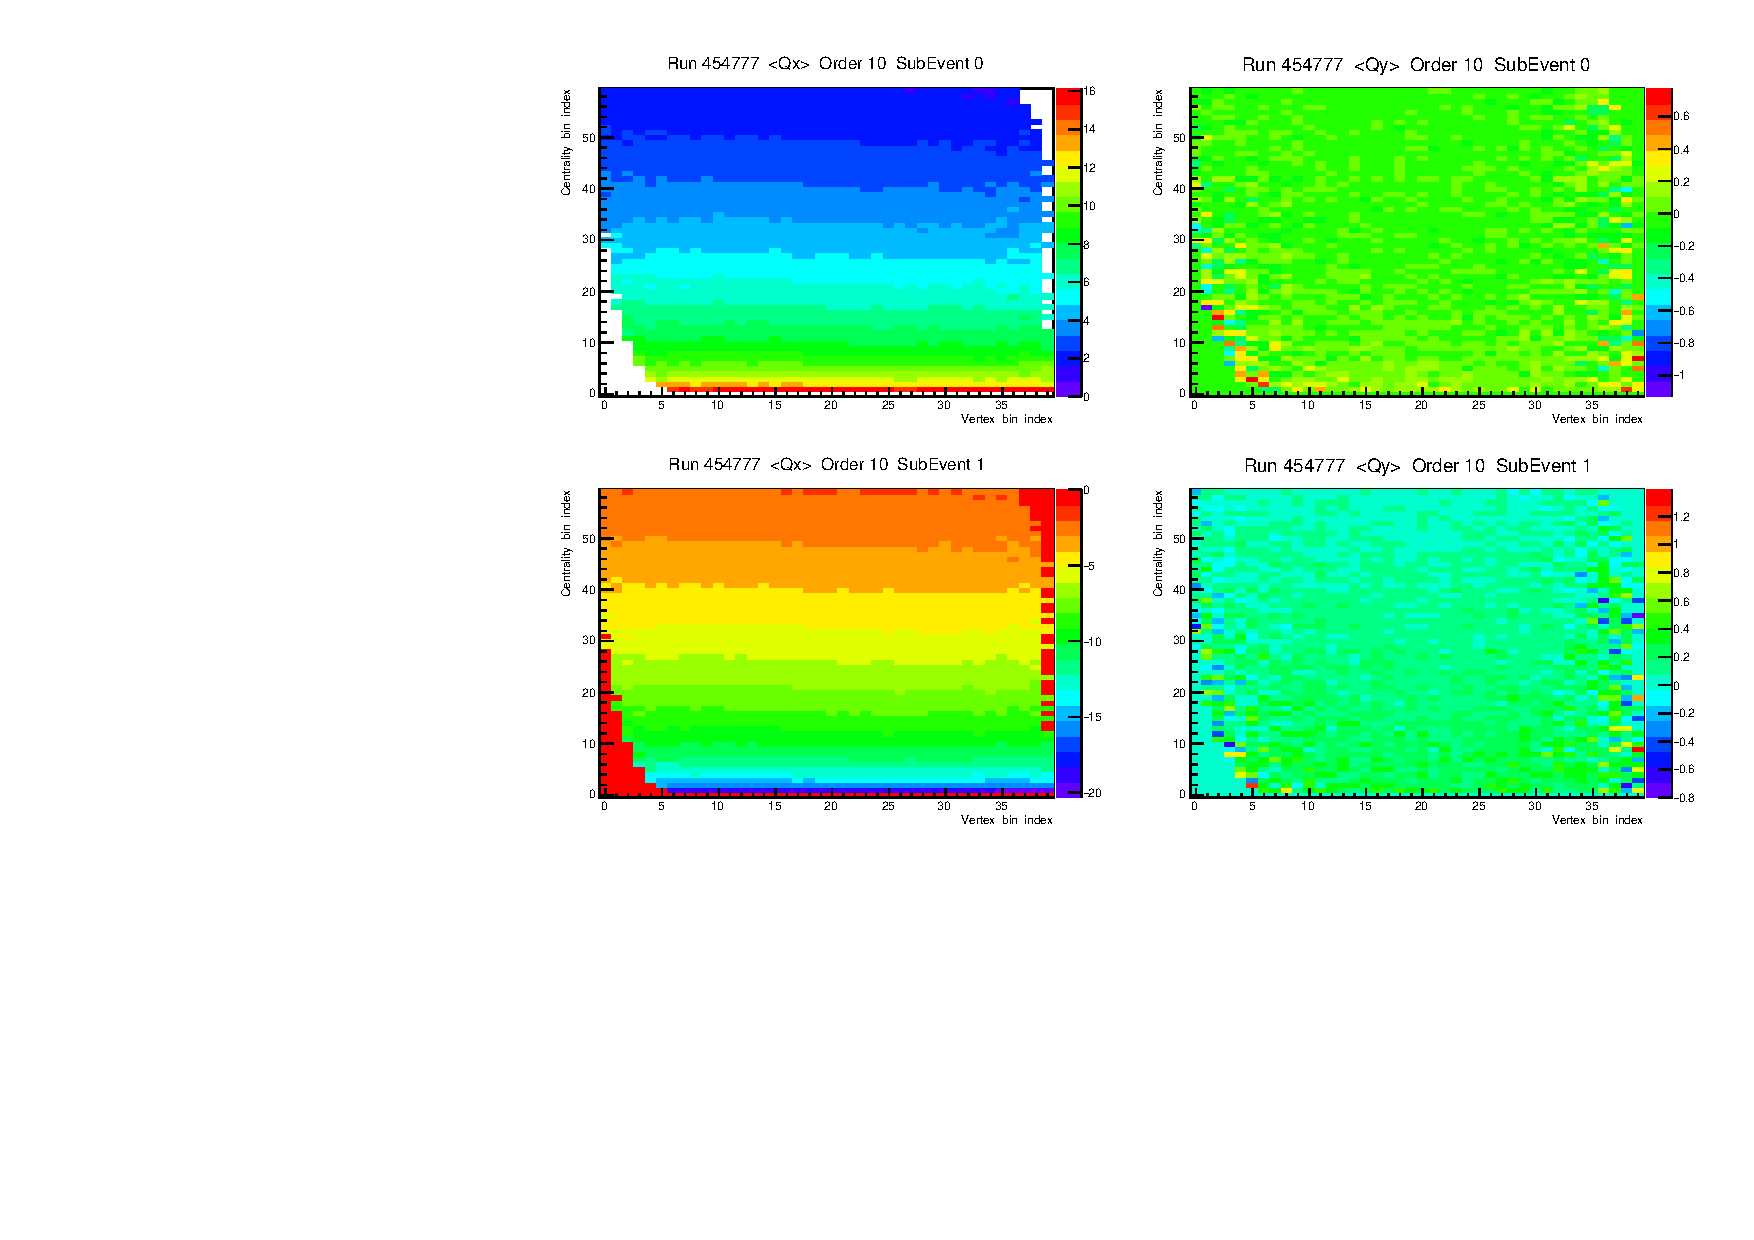
\includegraphics[width=0.7\textwidth]{fig_eventplane/QC_454777_ORD7.pdf}
\label{fig.bbc.qc7}
\caption{Non-normalized coefficients for Q$_{10}$ vector centering for BBC Run 454777 as a function of centrality and vertex bin. The top panels correspond to subevent 0 and the bottom panels correspond to subevent 1. The nominal vertex z=0 sits at around bin index 20 in the X axis.}
\end{figure}
\begin{figure}
\centering
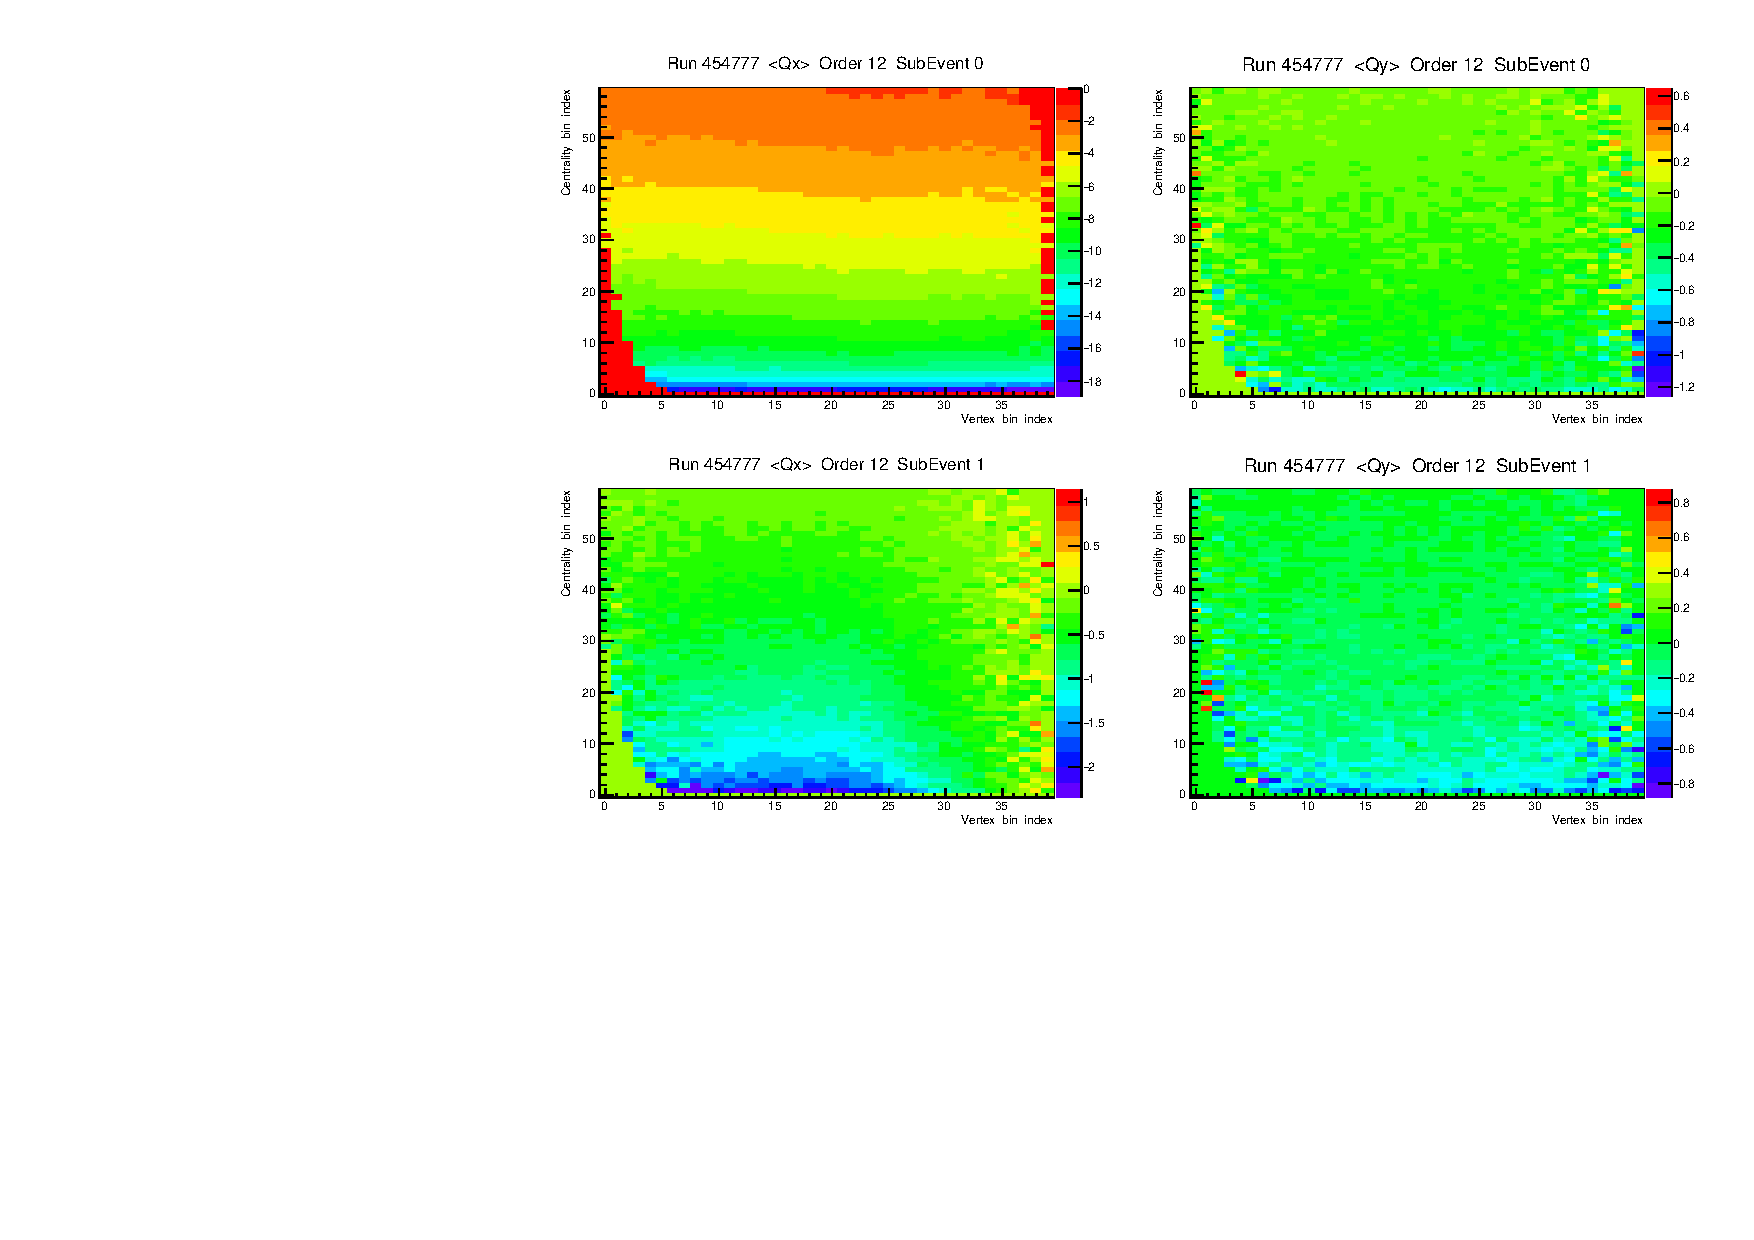
\includegraphics[width=0.7\textwidth]{fig_eventplane/QC_454777_ORD8.pdf}
\label{fig.bbc.qc8}
\caption{Non-normalized coefficients for Q$_{12}$ vector centering for BBC Run 454777 as a function of centrality and vertex bin. The top panels correspond to subevent 0 and the bottom panels correspond to subevent 1. The nominal vertex z=0 sits at around bin index 20 in the X axis.}
\end{figure}

The south arm (Au-going direction) was used for the symmetry angle determination.
The BBC south arm was subdivided into two subevents as shown in figure \ref{fig.bbcgeo}.
The calibration of the adc signal for the BBC is loaded from the general database code AAAAA.
On the other hand in order to eliminate potential biases for the BBC Q vectors the procedure described in section 2.
The calibration was done in bins of centrality and vertex; and was performed for every run of the entire used dataset.

Figure \ref{fig.bbc.qc1} shows the matrix of non-normalized {\bf centering coefficients} of Q$_2$ for one particular run of run 16 dAu 200 GeV corresponding to each subdivision of the BBC south. The X axis correspond to "Vertex Bin Index", where Z$_{vtx}=0$ is at idx=20 and spanning $dZ=1$ cm per bin. The Y axis corresponds to centrality. The Z axis is the average Qx (or Qy) which is denoted in color code. The matrix presents a high asymmetry with respect to Z$_{vtx}=0$  due to the collision asymmetric configuration and nominal position of the real interaction. The matrix for all other harmonics from 1 to 12 are displayed in figures from \ref{fig.bbc.qc0} to \ref{fig.bbc.qc8}.

Figure \ref{fig.bbc123} shows the {\bf symmetry angle} distribution for all events recorded in centrality 0-5 \%.
Each plot shows the effects of the calibration step by step from centering to flattening as discussed in the previous section in different colors.
The plots are arranged in a matrix for which the first two columns correspond to different sub events and the third column to the full event.
The first row of plots corresponds to the first order symmetry angle; the second column corresponds to the second order symmetry angle; while the third row, to the third order symmetry angle.
The distributions in blue are the raw distribution. As one can see centering diminishes most of the non-uniformities down to bellow 10\% in flatness. The next being scaling, down to below 3\%. This first stages take into account the acceptance and displacement of the bbc with respect of the event collision vertex.
Flattening being the last stage which leaves it to much below 1\% depending on the Q vector order.

\begin{figure}
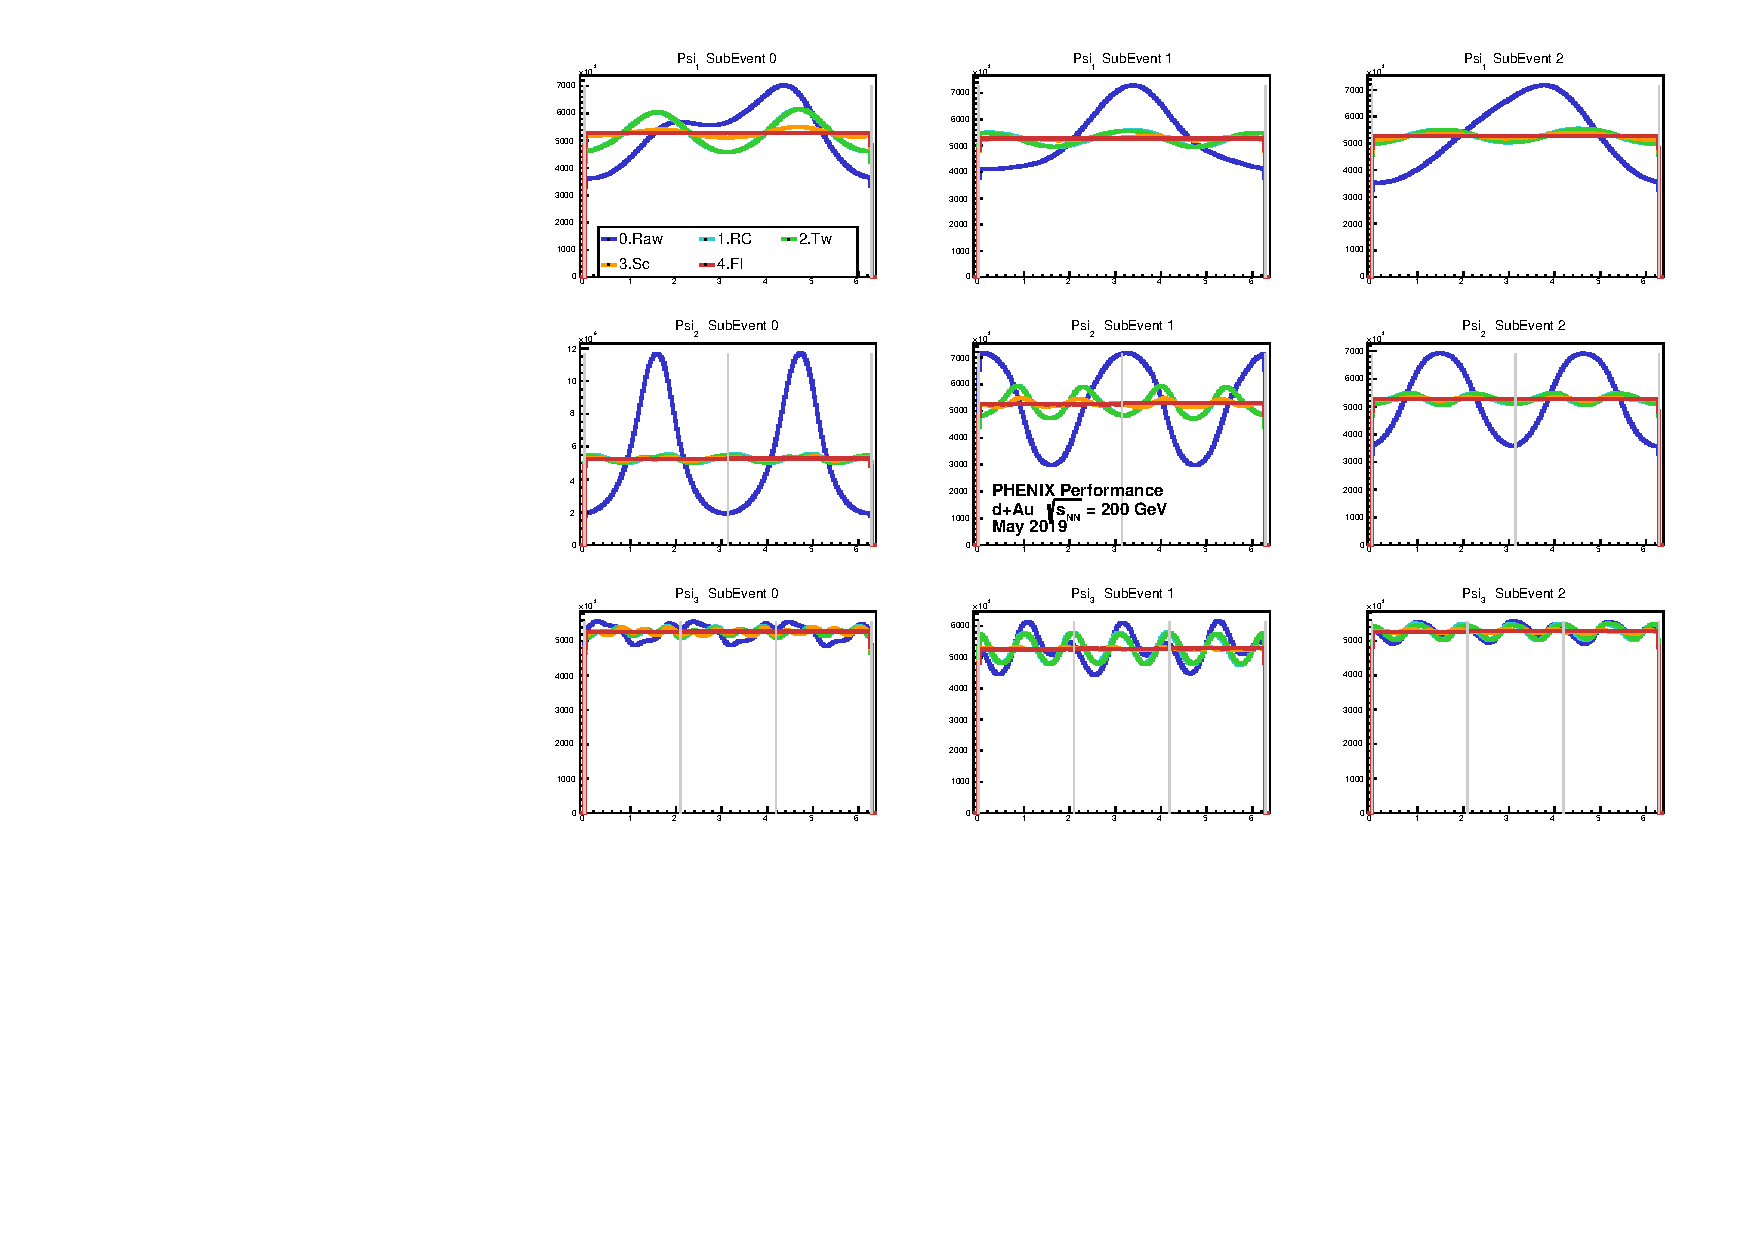
\includegraphics[width=\textwidth]{fig_eventplane/BBC123.pdf}
\label{fig.bbc123}
\caption{Symmetry angle measured by BBC-south detector for 0-5\% centrality events in d+Au collisions at 200 GeV. Order 1st, 2nd and 3rd}
\end{figure}
\begin{figure}
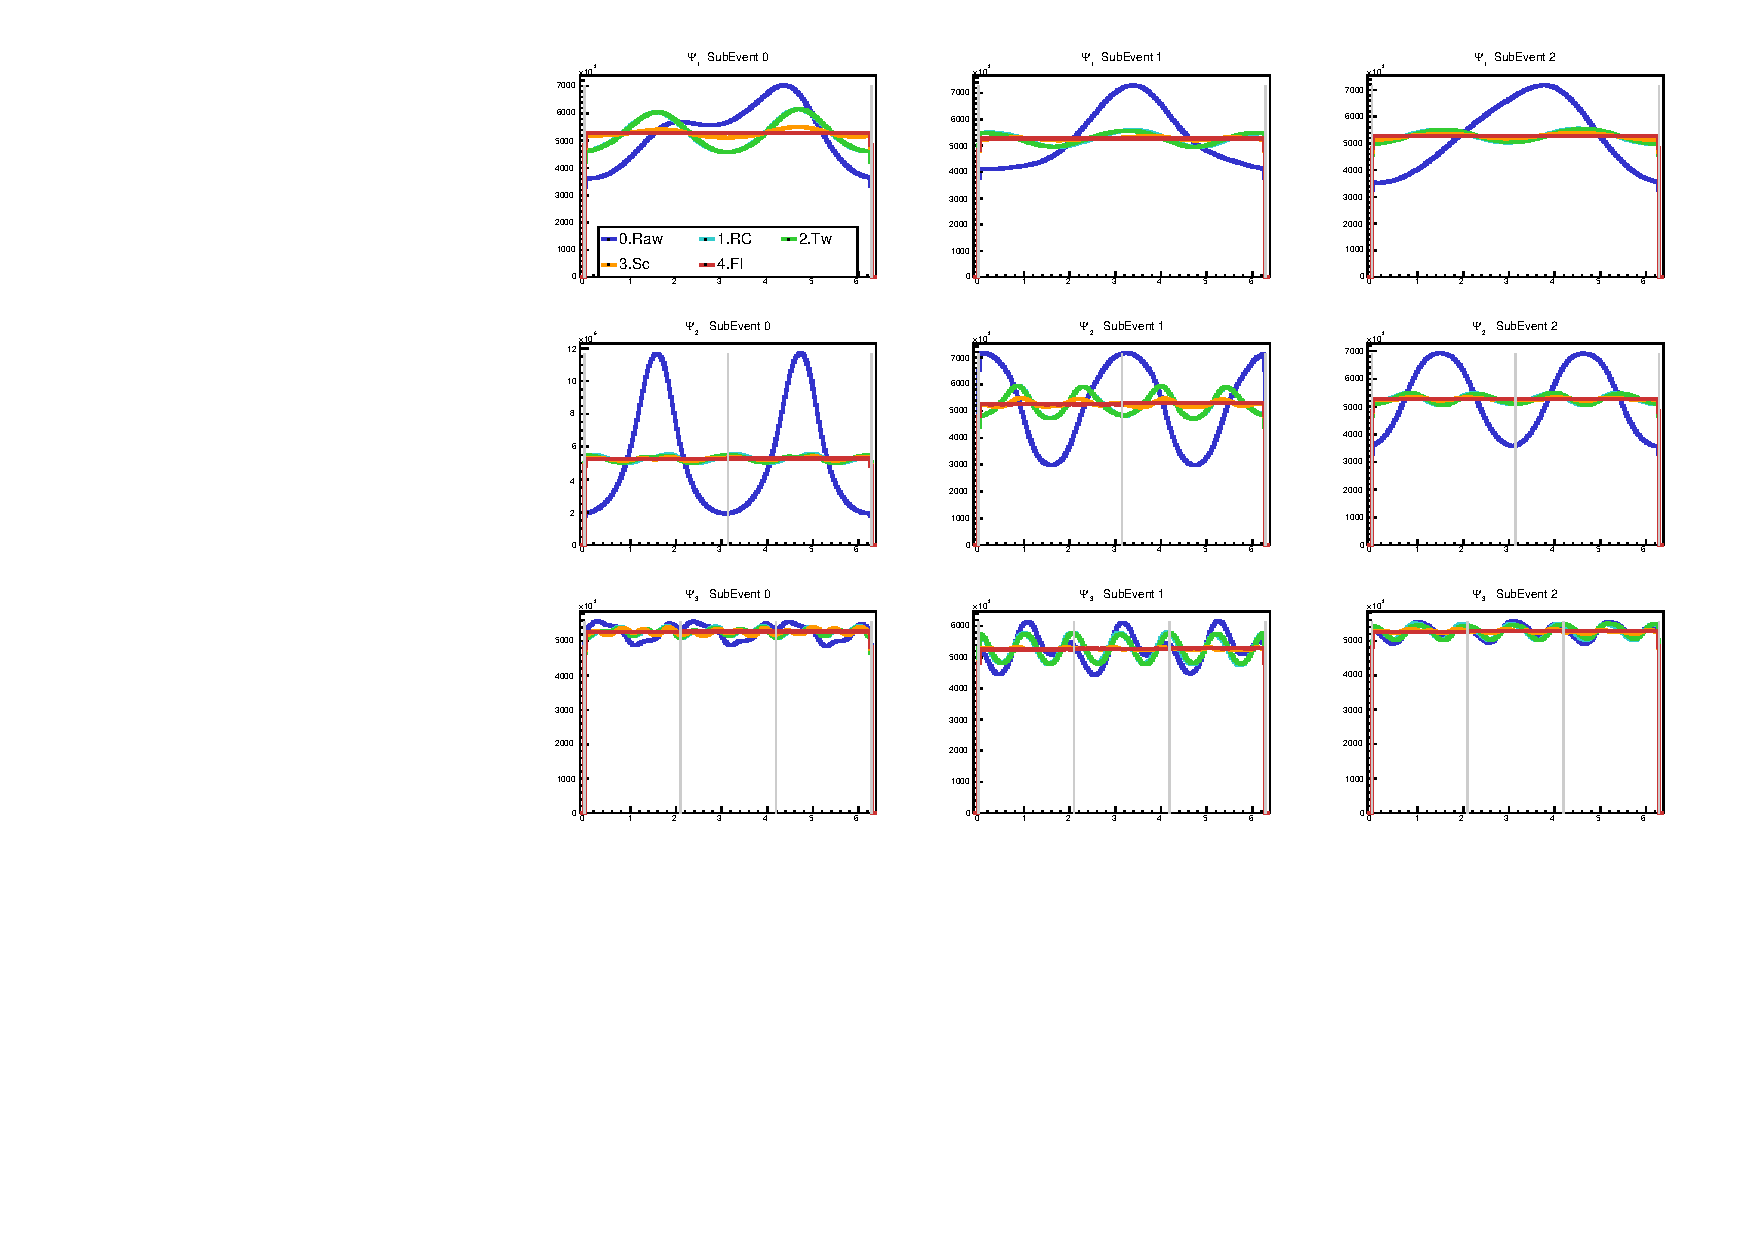
\includegraphics[width=\textwidth]{fig_eventplane/BBC456.pdf}
\label{fig.bbc456}
\caption{Symmetry angle measured by BBC-south detector for 0-5\% centrality events in d+Au collisions at 200 GeV. Order 4th, 5th and 6th}
\end{figure}

\bibliography{references}{}
\bibliographystyle{plain}
\end{document}
